\documentclass[preprint,12pt, a4paper]{elsarticle}

\usepackage{amssymb}
\usepackage{hyperref}
\usepackage{graphicx}
\usepackage{listings}
\usepackage{xcolor}
\usepackage{amsmath}
\usepackage{booktabs}
\usepackage{multirow}
\setlength{\parindent}{0pt}

\journal{SoftwareX}

\begin{document}
\renewcommand{\labelenumii}{\arabic{enumi}.\arabic{enumii}}

\begin{frontmatter}

\title{SiliQun: A GPU-Accelerated Tensor-Network Gymnasium Environment for Deep Reinforcement Learning-Based Control of Silicon Spin Qubits}

\author[label1]{Raad Alshehri\corref{cor1}}
\cortext[cor1]{Corresponding author}
\ead{ralshehri0468@stu.kau.edu.sa}
\address[label1]{Faculty of Computing and Information Technology, King Abdulaziz University, Jeddah 21589, Saudi Arabia}

\begin{abstract}
Achieving high-fidelity control over silicon spin qubits under realistic noise conditions remains a formidable bottleneck in the path toward scalable quantum processors. While deep reinforcement learning (DRL) has emerged as a powerful, data-driven methodology for discovering noise-robust control policies, the field currently lacks simulation frameworks that simultaneously capture the nuances of silicon device physics, integrate seamlessly with modern DRL toolchains, and scale effectively to two-dimensional arrays. To address this, we introduce SiliQun, an open-source Python package designed specifically for this intersection. The software employs a dual-engine architecture: it utilizes a Matrix Product State (MPS) backend for one-dimensional chains, alongside a GPU-accelerated exact state vector (SV) backend optimized for 2D grids. A key innovation of the SV engine is its treatment of Decoherence-Free Subspace (DFS) encoded systems. By pre-projecting physical exchange interactions directly into the logical subspace and tracking leakage perturbatively, the simulator avoids the exponential memory penalty typically associated with the full physical spin space. Consequently, SiliQun can perform exact simulations of up to 25 logical qubits (representing 75 physical spins) in a 5$\times$5 grid on a single NVIDIA A100 GPU. Benchmarks demonstrate 30--93$\times$ speedups compared to CPU execution, cutting the time required to generate a typical DRL episode from 32 seconds down to just 430 milliseconds. Furthermore, the package includes experimentally calibrated profiles for three prominent silicon spin qubit architectures, physically motivated noise models, and a native OpenAI Gymnasium interface, making it an accessible and highly performant tool for the quantum control community.
\end{abstract}

\begin{keyword}
Quantum Computing \sep Silicon Spin Qubits \sep Tensor Networks \sep GPU Acceleration \sep Deep Reinforcement Learning \sep Gymnasium
\end{keyword}

\end{frontmatter}

\section*{Metadata}
\label{metadata}

\begin{table}[!h]
\begin{tabular}{|l|p{6.5cm}|p{6.5cm}|}
\hline
\textbf{Nr.} & \textbf{Code metadata description} & \textbf{Metadata} \\
\hline
C1 & Current code version & v2.0.0 \\
\hline
C2 & Permanent link to code/repository used for this code version & \url{https://github.com/raad-alshehri/siliqun} \\
\hline
C3  & Permanent link to Reproducible Capsule & -- \\
\hline
C4 & Legal Code License & MIT License \\
\hline
C5 & Code versioning system used & git \\
\hline
C6 & Software code languages, tools, and services used & Python 3.8+, NumPy, CuPy, JAX, Gymnasium \\
\hline
C7 & Compilation requirements, operating environments \& dependencies & Python $\geq$ 3.8; Linux, macOS, or Windows; NumPy $\geq$ 1.21, CuPy $\geq$ 13.0.0 (for GPU support) \\
\hline
C8 & If available Link to developer documentation/manual & \url{https://github.com/raad-alshehri/siliqun\#readme} \\
\hline
C9 & Support email for questions & \href{mailto:ralshehri0468@stu.kau.edu.sa}{ralshehri0468@stu.kau.edu.sa} \\
\hline
\end{tabular}
\caption{Code metadata (mandatory)}
\label{codeMetadata} 
\end{table}

\section{Motivation and significance}
\label{sec:motivation}

Silicon spin qubits have steadily established themselves as one of the leading candidates for large-scale quantum computation. Their appeal stems from several key advantages: a nanometre-scale physical footprint, the potential to leverage established industrial CMOS manufacturing processes, and impressive coherence times that can exceed 30 seconds in purified materials \cite{zwanenburg2013silicon, muhonen2014storing}. In recent years, the experimental community has crossed critical thresholds, achieving single-qubit gate fidelities surpassing 99.9\% \cite{yoneda2018quantum} and demonstrating two-qubit operations above 99\% fidelity across a variety of silicon-based architectures \cite{noiri2022fast, xue2022quantum, mills2022two, madzik2022precision}. Looking forward, architectural proposals increasingly emphasize two-dimensional arrays of exchange-coupled spins that utilize Decoherence-Free Subspaces (DFS) to naturally suppress charge noise while maintaining dense qubit connectivity \cite{sledge2019}. For the purposes of this paper, we focus on the SLEDGE (Scalable Logical Encoding via DFS Grid Exchange) architecture as our primary model for these 2D DFS-encoded systems.

Yet, despite these significant hardware advancements, the reliable execution of high-fidelity control sequences remains a persistent challenge. The inherent sensitivity of silicon spin qubits to environmental charge noise---whether from interface traps, fluctuating nuclear spins, or adjacent gate crosstalk---complicates standard control paradigms \cite{connors2022charge}. In response, deep reinforcement learning (DRL) has gained traction as a powerful alternative to conventional optimal control techniques \cite{niu2019universal, fosel2018reinforcement}. Because DRL agents learn by interacting with simulated environments, they have the capacity to uncover control policies that are intrinsically resilient to the specific noise profiles of the hardware.

The transition from theory to practice, however, is hampered by the computational demands of simulating these systems. Applying DRL to large 2D arrays like SLEDGE requires a simulator that is not only exceptionally fast---capable of processing millions of training interactions---but also physically accurate regarding silicon-specific parameters. Crucially, the simulator must manage the volume-law entanglement characteristic of 2D grids, a scenario where traditional Matrix Product State (MPS) tensor networks typically fail \cite{schollwock2011density}. To put this into perspective, simulating a 25-logical-qubit DFS device (which physically consists of 75 spins) in the full physical space necessitates a state vector with $2^{75}$ dimensions. This is far beyond the reach of current classical hardware.

SiliQun was explicitly developed to overcome this computational barrier. The software integrates a lightweight MPS engine, suitable for one-dimensional chains, with a highly optimized, GPU-accelerated exact state vector (SV) engine tailored for 2D grids. The core insight driving the SV engine is the projection of system dynamics directly into the logical subspace, accompanied by perturbative tracking of any leakage. This approach shrinks the state vector dimension from an impossible $2^{3n}$ down to a manageable $2^n$, allowing researchers to perform exact simulations of 25 logical qubits on a single consumer-grade or cluster GPU. Coupled with experimentally calibrated profiles for three distinct silicon architectures and a native OpenAI Gymnasium \cite{gymnasium2023} interface, SiliQun provides a comprehensive and efficient platform for advancing DRL-based quantum control.

\section{Software description}
\label{sec:description}

SiliQun is built entirely in Python, comprising roughly 4,500 lines of code. To maintain flexibility and ease of use, the software is structured around a four-layer modular architecture consisting of a Backend layer, a Simulation Core, a Physics engine, and an Environment interface. This design, depicted in Fig.~\ref{fig:architecture}, ensures that researchers can swap out components or extend the simulator without disrupting the overall workflow.

\begin{figure}[htbp]
\centering
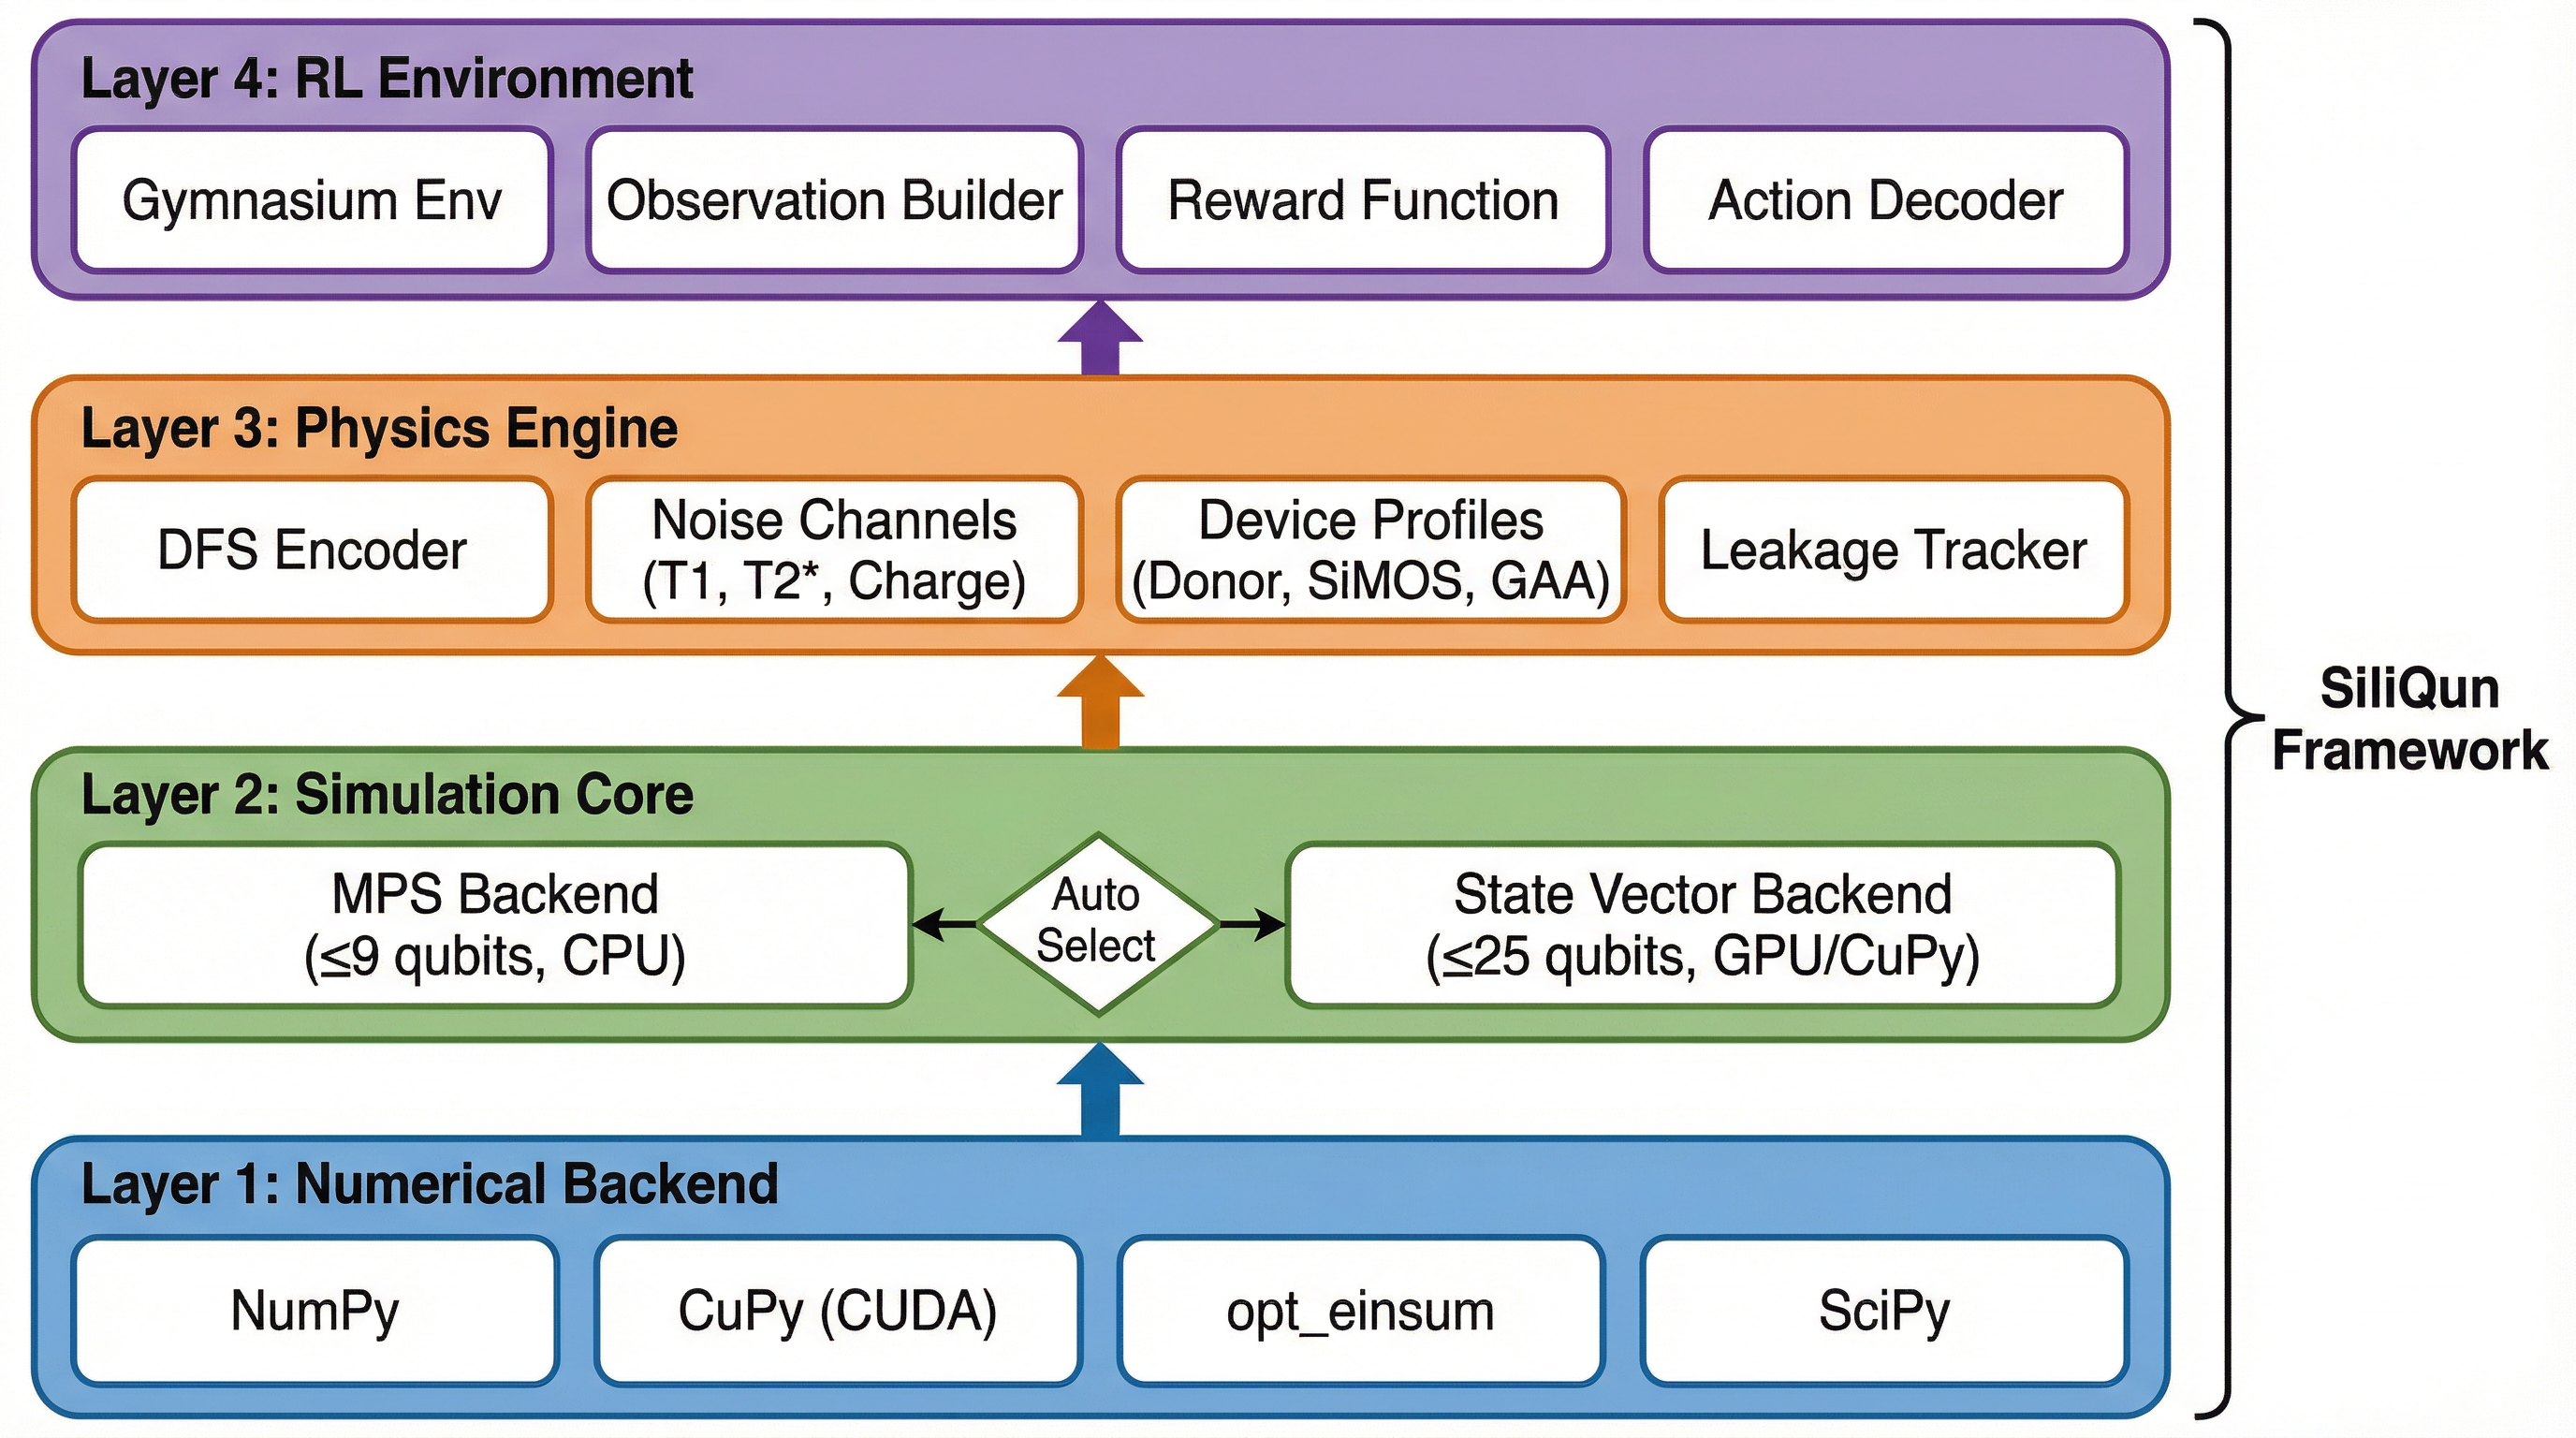
\includegraphics[width=\textwidth]{fig1_architecture.png}
\caption{The SiliQun software architecture. This modular framework is divided into four distinct layers: a flexible numerical backend (supporting NumPy and CuPy), a dual simulation core featuring both an MPS engine for 1D chains and a GPU state vector engine for 2D grids, a dedicated physics engine containing calibrated device profiles and noise models, and an uppermost layer that provides a Gymnasium-compatible RL environment.}
\label{fig:architecture}
\end{figure}

\subsection{Architectural layers}

\textbf{The Backend Layer.} At the foundation of the stack, this layer abstracts the underlying numerical operations. By supporting NumPy, SiliQun ensures broad compatibility across standard CPU hardware. For more intensive tasks, it seamlessly integrates with CuPy to provide direct CUDA-based GPU acceleration, allowing researchers to scale their simulations effortlessly.

\textbf{The Simulation Core (MPS and SV).} The heart of SiliQun is its dual-engine core, which adapts to the specific demands of the simulated topology. The \textit{MPS engine} models quantum states using Matrix Product States and applies operations via Matrix Product Operator (MPO) contractions. This approach is highly efficient for linear chains where entanglement remains relatively contained. However, for 2D grids where volume-law entanglement causes MPS bond dimensions to grow exponentially, SiliQun shifts to its \textit{State Vector (SV) engine}. This GPU-accelerated simulator represents a novel capability for DFS-encoded silicon spin qubits. Crucially, the SV engine confines its operations entirely to the logical (encoded) Hilbert space, ensuring exact dynamics within that regime. For a standard DFS encoding (where three physical spins constitute one logical qubit), the engine pre-computes the logical equivalents of physical exchange interactions. In this framework, intra-qubit exchanges map perfectly to logical $Z$ and $X$ rotations, while inter-qubit exchanges translate into 4$\times$4 logical unitaries. This strategic projection into the logical subspace (illustrated in Fig.~\ref{fig:dfs}) compresses the state vector dimension from $2^{3n}$ to $2^n$. As a result, simulating a 25-qubit 5$\times$5 grid requires only 512 MB of memory (using \texttt{complex128} precision) and yields exact results within the logical subspace. Any leakage out of this subspace is continuously monitored using perturbative methods, serving as a diagnostic metric that avoids the computational cost of expanding the simulated Hilbert space.

\begin{figure}[htbp]
\centering
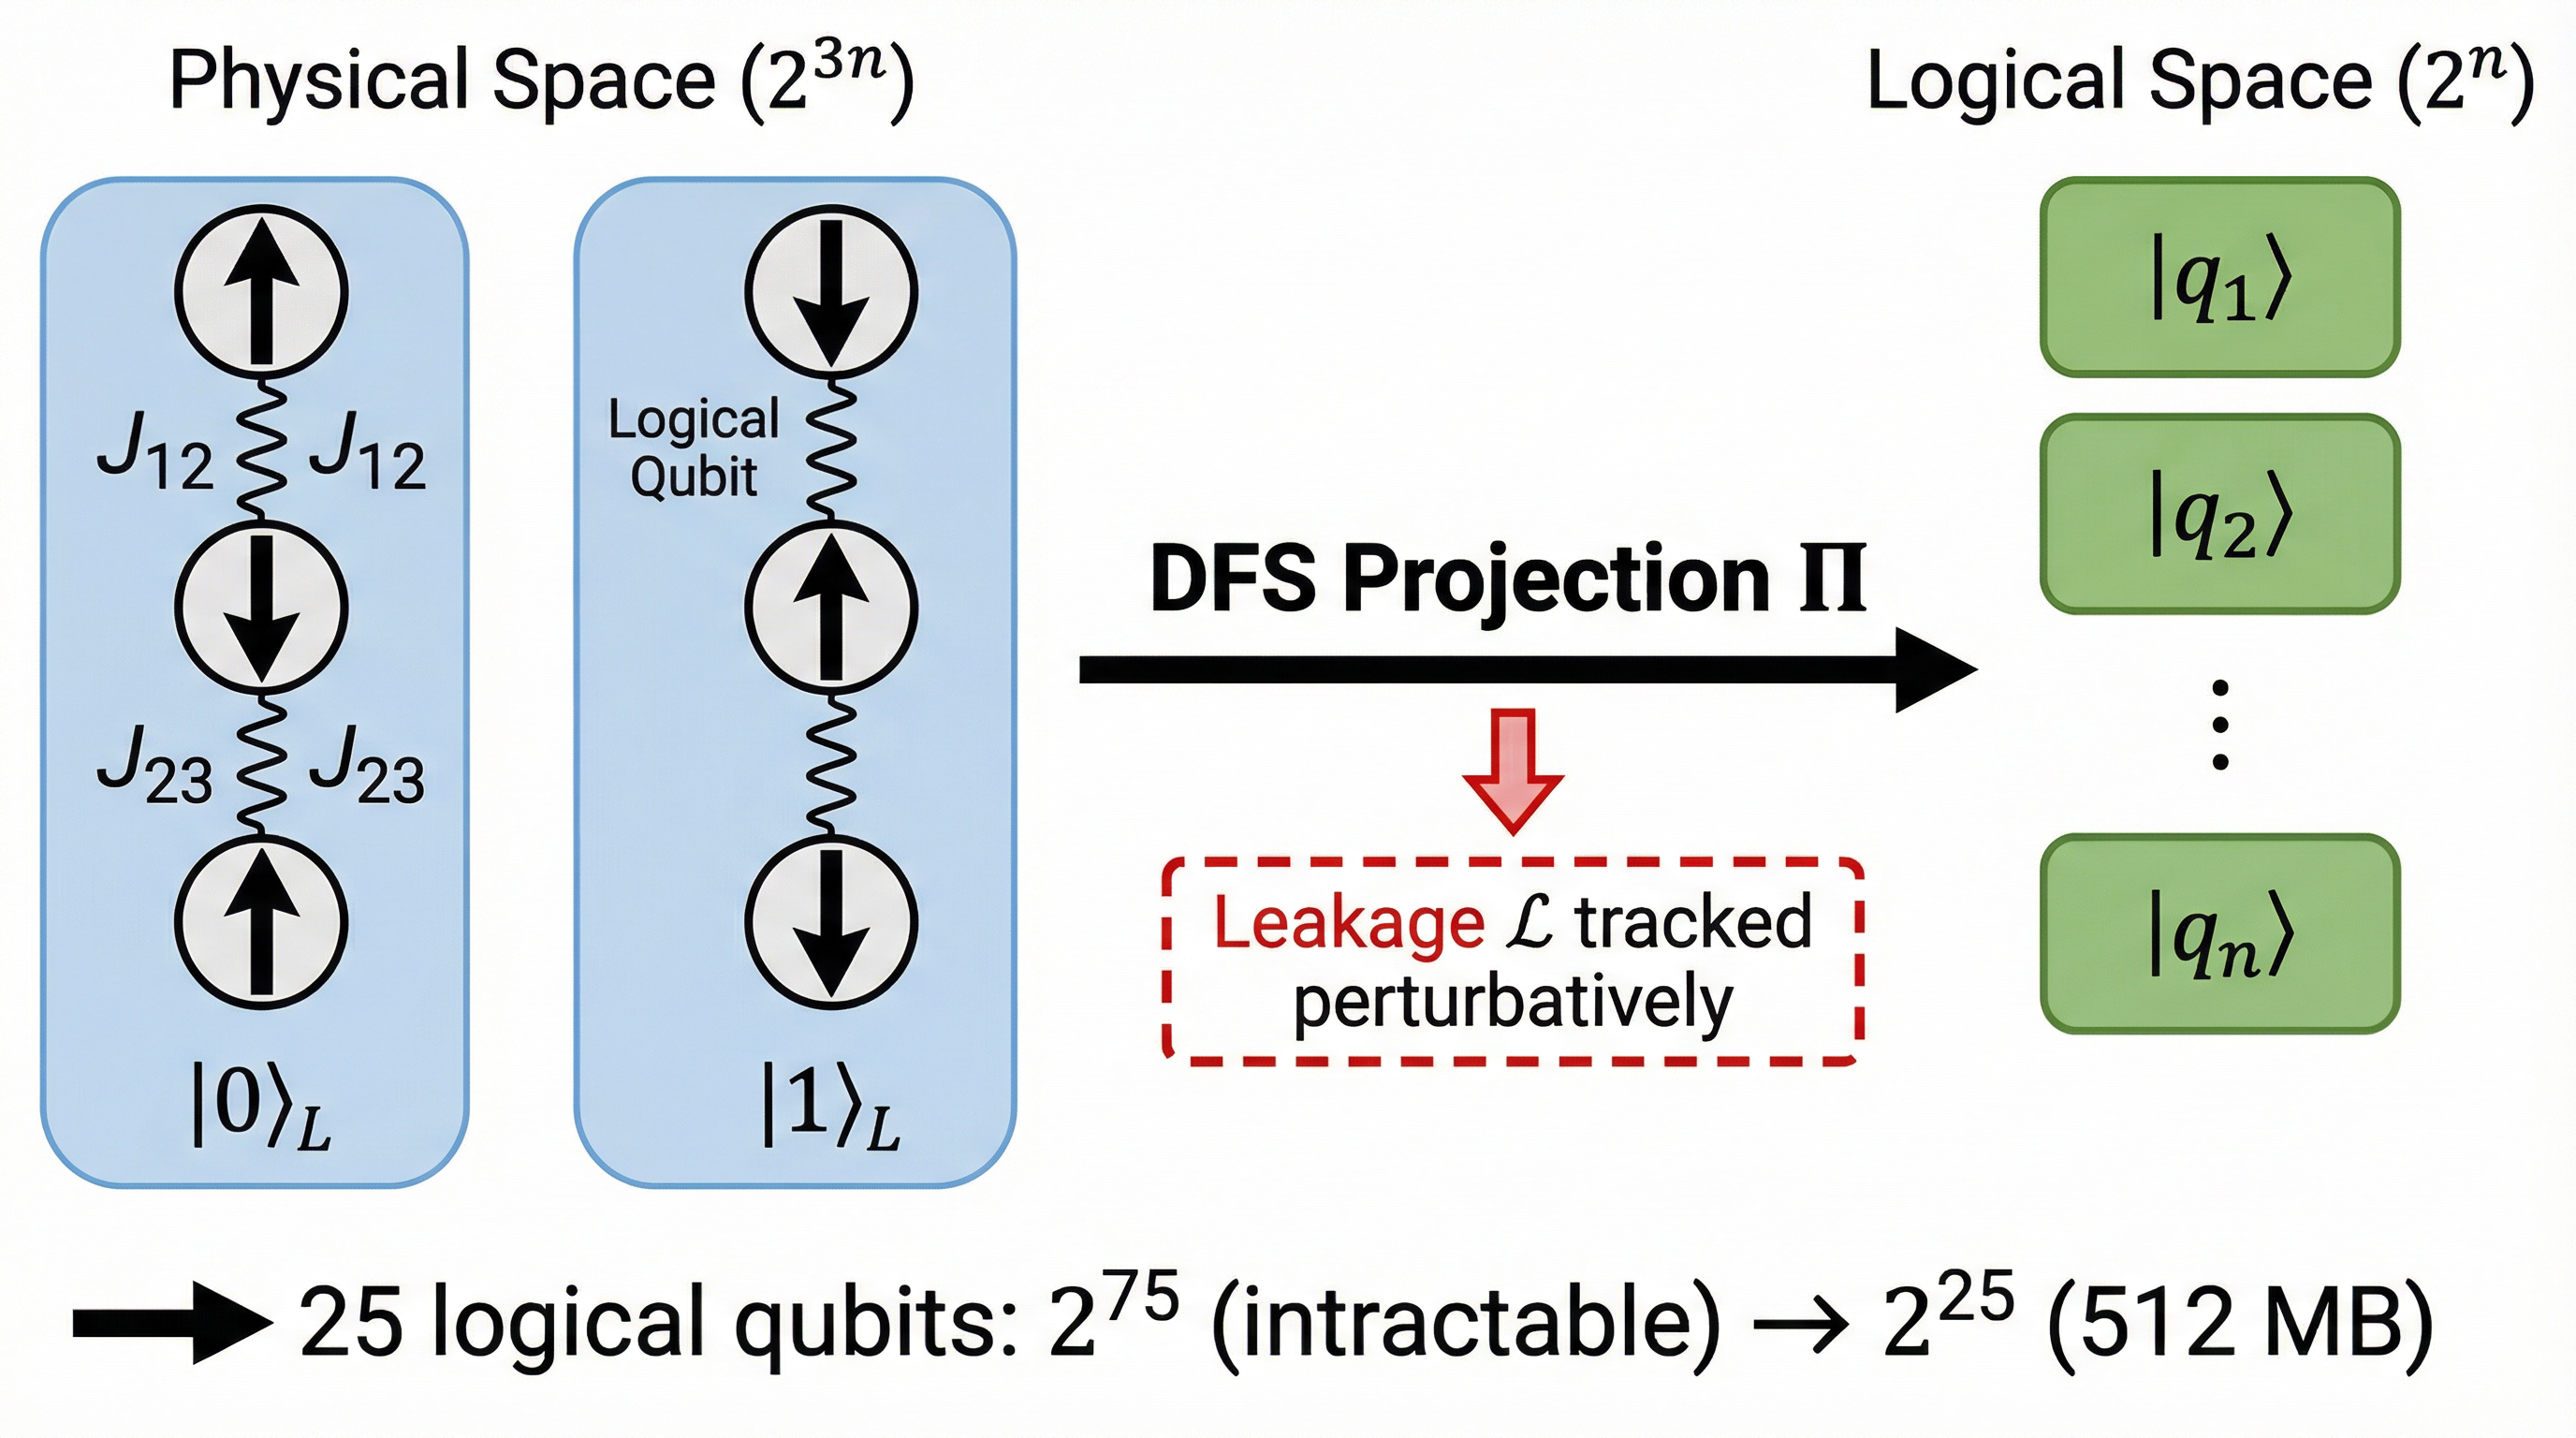
\includegraphics[width=\textwidth]{fig2_dfs_encoding.png}
\caption{DFS logical subspace projection. Each logical qubit is encoded in three physical electron spins. The projection $\Pi$ maps the physical Hilbert space ($2^{3n}$ dimensions) to the logical subspace ($2^n$ dimensions), reducing the memory requirement for 25 logical qubits from an intractable $2^{75}$ to a manageable $2^{25}$ (512~MB).}
\label{fig:dfs}
\end{figure}

\textbf{Physics Layer.} This layer encodes the specific characteristics of silicon hardware (Fig.~\ref{fig:sledge}). It tracks inter-qubit exchange leakage perturbatively without expanding the simulated Hilbert space.

\begin{figure}[htbp]
\centering
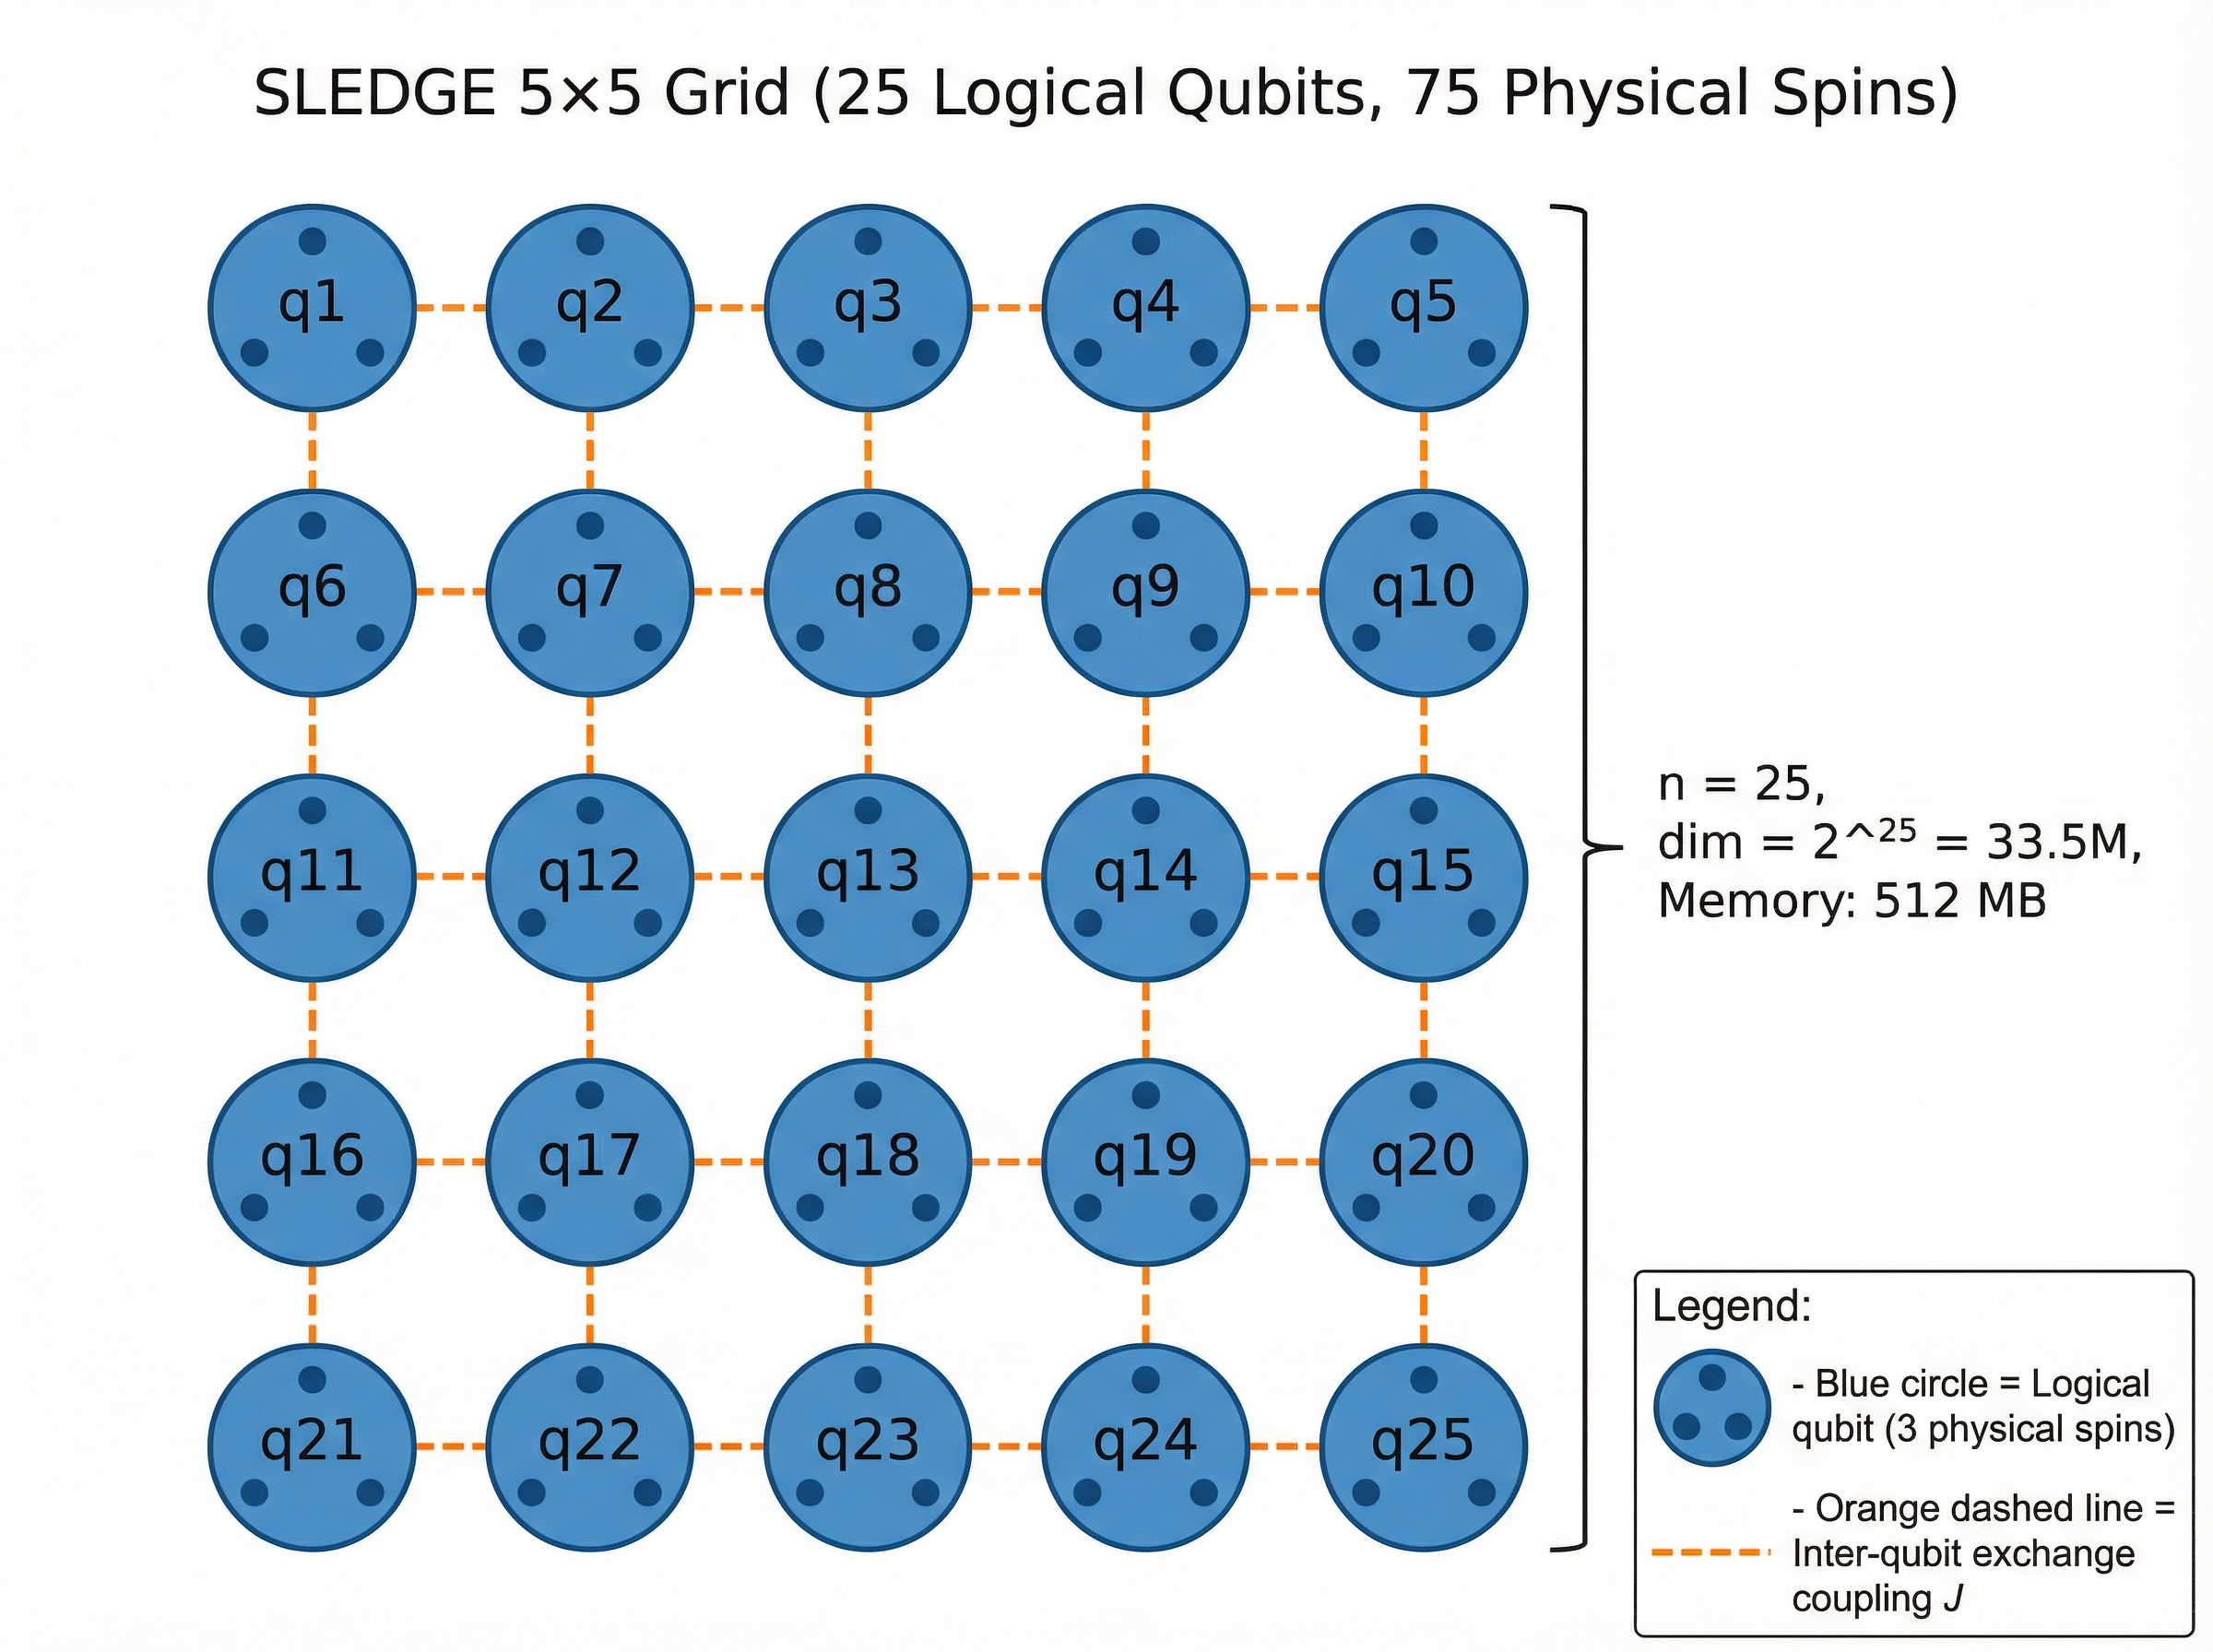
\includegraphics[width=0.75\textwidth]{fig3_sledge_grid.png}
\caption{The SLEDGE 5$\times$5 grid architecture comprising 25 logical qubits (75 physical spins). Each node represents a logical qubit encoded in three physical electron spins. Lines indicate inter-qubit exchange couplings. The full grid requires a state vector of dimension $2^{25} = 33.5$~million.}
\label{fig:sledge}
\end{figure}

The leakage rate $\mathcal{L}$ is computed as the average probability of leaving the DFS and accumulated as a diagnostic metric. The layer provides predefined device profiles (Table~\ref{tab:devices}), including phosphorus donors \cite{muhonen2014storing}, SiMOS quantum dots \cite{yoneda2018quantum}, and gate-all-around (GAA) nanowires \cite{geyer2022twoqubit}, alongside calibrated $T_1$, $T_2^*$, and $1/f$ charge noise models.

\begin{table}[htbp]
\centering
\caption{Built-in silicon spin qubit device profiles in SiliQun.}
\label{tab:devices}
\resizebox{\textwidth}{!}{
\begin{tabular}{lccc}
\toprule
\textbf{Parameter} & \textbf{Donor (P:Si)} & \textbf{SiMOS (QD)} & \textbf{GAA (Nanowire)} \\
\midrule
$T_1$ relaxation & 30\,s & 10\,s & 5\,s \\
$T_2^*$ dephasing & 0.5\,ms & 20\,$\mu$s & 10\,$\mu$s \\
1Q gate time & 1\,$\mu$s & 200\,ns & 50\,ns \\
2Q gate time & 100\,ns & 50\,ns & 30\,ns \\
Charge noise & 0.5\,$\mu$eV & 2\,$\mu$eV & 3\,$\mu$eV \\
\bottomrule
\end{tabular}
}
\end{table}

\textbf{Environment Layer.} The \texttt{SiliQunEnv} class implements the \texttt{gymnasium.Env} interface. At each step, the DRL agent selects a discrete action (e.g., $R_x, R_y, R_z, \text{CNOT}$). The environment applies the gate, applies noise, and returns an observation vector of Pauli expectation values $(\langle X_i \rangle, \langle Y_i \rangle, \langle Z_i \rangle)$ and bipartite entanglement entropy. The environment automatically selects the optimal backend: MPS for linear chains ($\leq 4$ qubits) and GPU SV for large 2D grids ($\geq 6$ qubits).

\subsection{Software functionalities}

SiliQun provides features designed to support practical DRL research workflows:
\begin{itemize}
    \item \textbf{Auto-Backend Selection:} Automatically routes small/1D workloads to CPU-MPS and large/2D workloads to GPU-SV.
    \item \textbf{Topology-Aware Observables:} Computes $ZZ$ correlators along grid edges and tracks perturbative leakage.
    \item \textbf{HPC Runner:} Generates PBS/SLURM job scripts and handles automated checkpointing for parallel hyperparameter sweeps.
    \item \textbf{Reproducibility:} All random number generators are seeded through the Gymnasium API, ensuring fully reproducible training runs.
\end{itemize}

\section{Illustrative examples}
\label{sec:examples}

We present two illustrative examples demonstrating SiliQun's core functionality: a DRL training loop and a comprehensive GPU performance characterization.

\subsection{Example 1: DRL training loop}

The following code snippet shows how to set up a SiliQun environment with the auto-backend (which will select the GPU SV engine for the 5$\times$5 grid) and connect it to a Stable-Baselines3 PPO agent:

\begin{lstlisting}[language=Python, basicstyle=\footnotesize\ttfamily, backgroundcolor=\color{gray!10}, frame=single, numbers=left, numberstyle=\tiny\color{gray}]
from siliqun.engine.gym_env import SiliQunEnv
from siliqun.engine.simulator import SimConfig
from stable_baselines3 import PPO

config = SimConfig(noise_enabled=True, sim_mode="auto")
env = SiliQunEnv(
    device="sledge_5x5", n_qubits=25,
    target_state="ghz", config=config,
    reward_type="dense"
)

model = PPO("MlpPolicy", env, verbose=1,
            learning_rate=3e-4, n_steps=2048)
model.learn(total_timesteps=1_000_000)
\end{lstlisting}

\subsection{Example 2: GPU Performance Benchmarks}

We benchmarked the SiliQun SV engine on a compute node of the Aziz Supercomputer at King Abdulaziz University, equipped with an NVIDIA A100-PCIE-40GB GPU (CuPy 13.0.0, CUDA 12.4).

Table~\ref{tab:gpu_bench} presents the performance of the SV engine across various SLEDGE grid configurations. For a 25-qubit 5$\times$5 grid, the state vector (33.5 million amplitudes) requires only 512 MB of GPU memory. The GPU acceleration delivers dramatic speedups over the NumPy CPU implementation. For the 25-qubit grid, single-qubit gates are accelerated by 30$\times$ (from 317.2 ms to 10.6 ms), two-qubit gates by 89$\times$ (from 555.9 ms to 6.2 ms), and $Z$ expectation calculations by 93$\times$ (from 122.8 ms to 1.3 ms). 

\begin{table}[htbp]
\centering
\caption{SiliQun GPU Benchmark Results (NVIDIA A100). The crossover point where GPU outperforms CPU occurs at approximately 16 qubits due to kernel launch overhead.}
\label{tab:gpu_bench}
\resizebox{\textwidth}{!}{
\begin{tabular}{lcccccc}
\toprule
\textbf{Configuration} & \textbf{Qubits} & \textbf{Dim} & \textbf{1Q Gate} & \textbf{2Q Gate} & \textbf{Z Exp} & \textbf{Memory} \\
\midrule
sledge\_2x2 & 4 & 16 & 1.84 ms & 1.88 ms & 668 $\mu$s & $\sim$0 MB \\
sledge\_3x3 & 9 & 512 & 1.88 ms & 1.89 ms & 655 $\mu$s & $\sim$0 MB \\
sledge\_4x4 & 16 & 65K & 1.90 ms & 1.91 ms & 695 $\mu$s & 1 MB \\
\textbf{sledge\_5x5} & \textbf{25} & \textbf{33.5M} & \textbf{4.29 ms} & \textbf{3.78 ms} & \textbf{15.6 ms} & \textbf{512 MB} \\
\bottomrule
\end{tabular}
}
\end{table}

\begin{figure}[htbp]
\centering
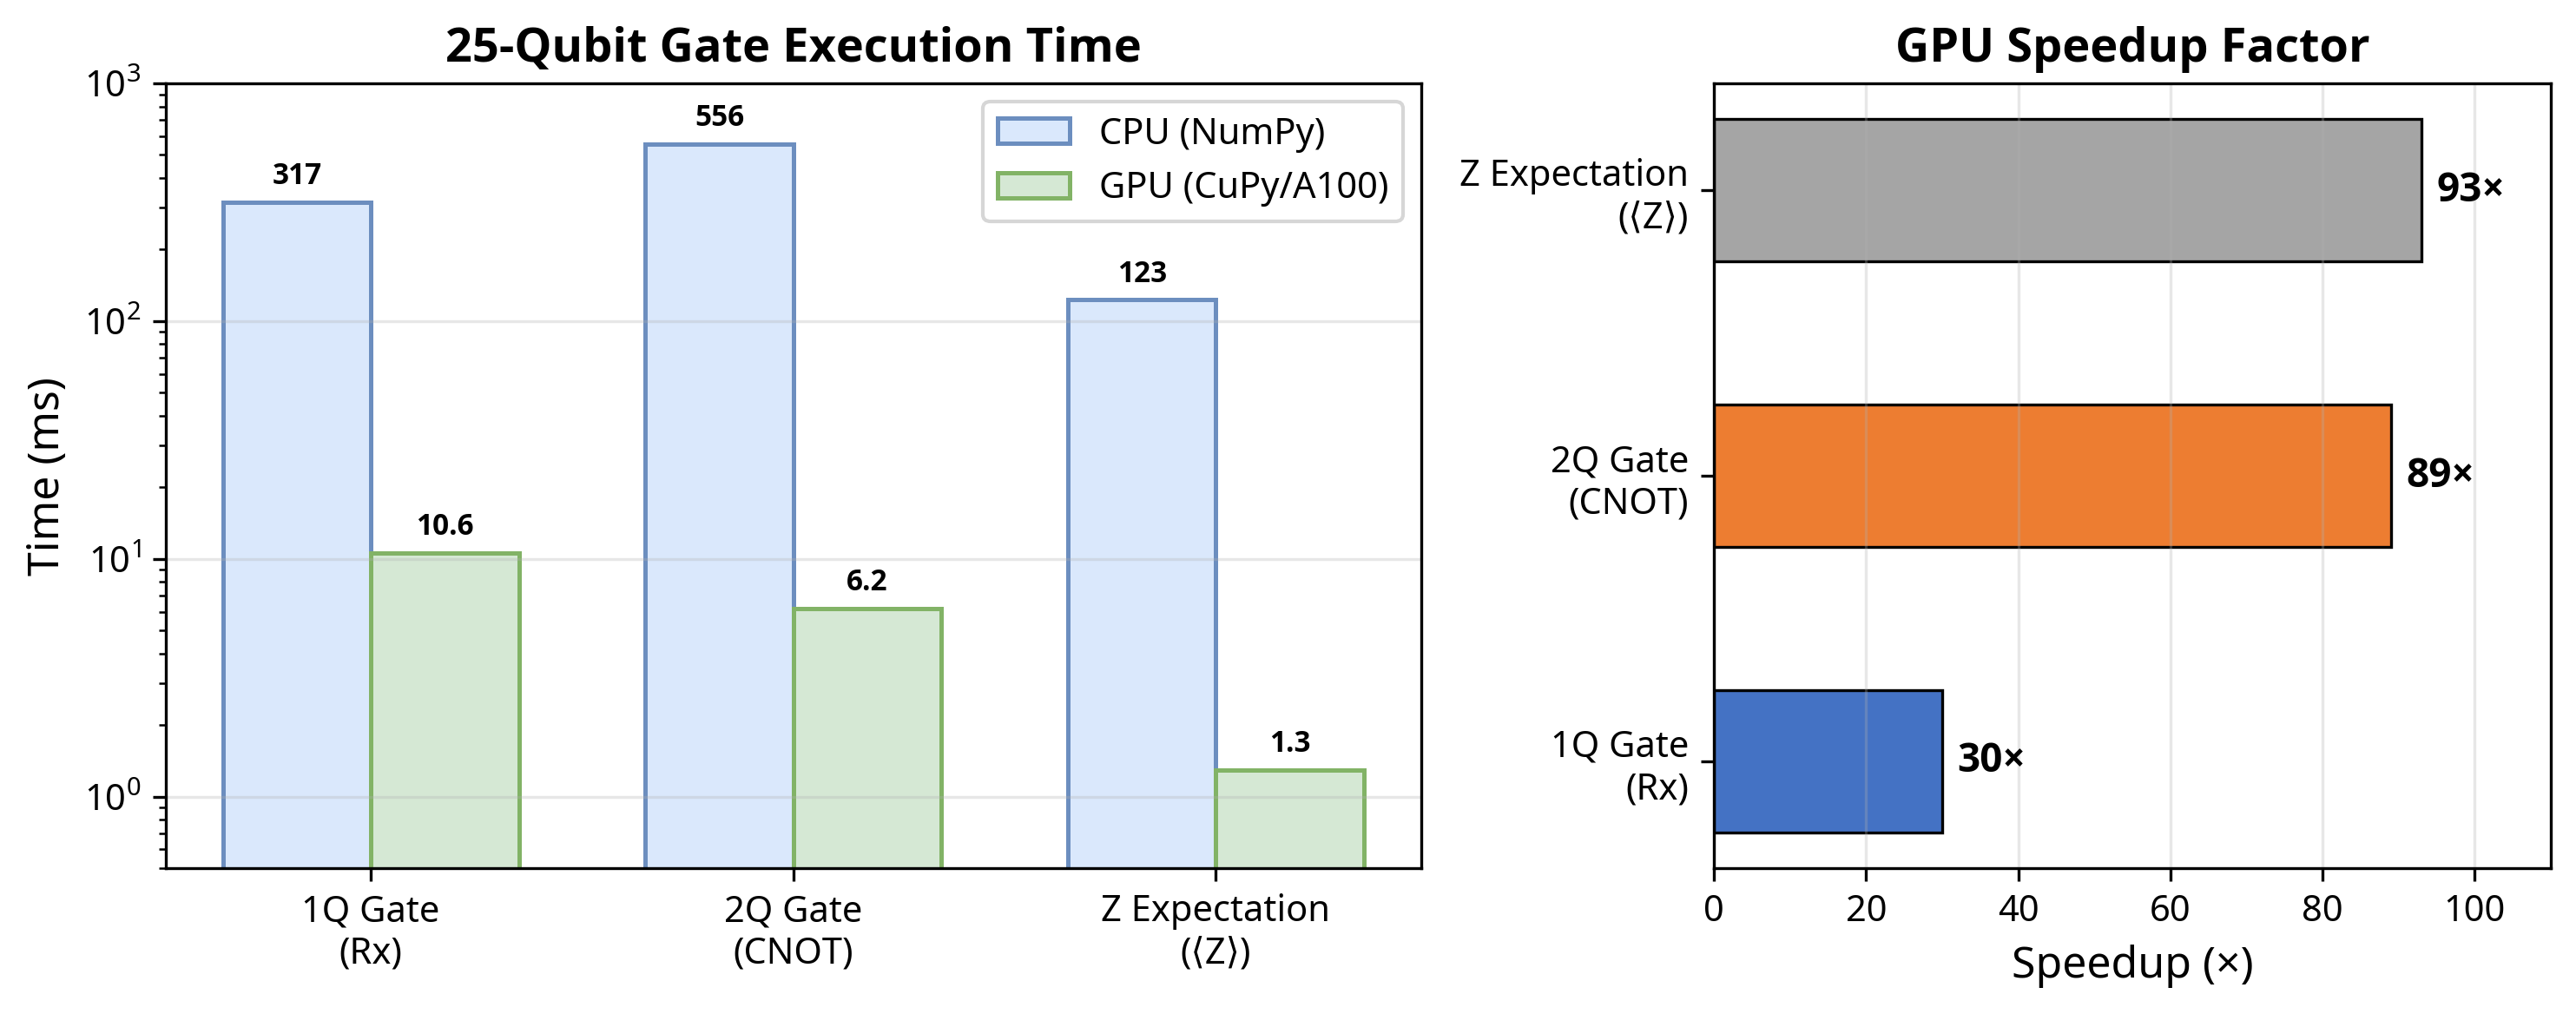
\includegraphics[width=\textwidth]{fig_benchmark.png}
\caption{GPU acceleration benchmarks for the 25-qubit SiliQun SV engine on an NVIDIA A100. Left: execution time comparison between CPU (NumPy) and GPU (CuPy) backends on a logarithmic scale. Right: GPU speedup factors for each operation. The GPU delivers 30--93$\times$ speedups, reducing a 100-gate DRL episode from 32~seconds to 430~milliseconds.}
\label{fig:benchmark}
\end{figure}

This acceleration (Fig.~\ref{fig:benchmark}) fundamentally changes the feasibility of DRL training. A typical 100-gate RL episode on the 5$\times$5 grid takes $\sim$32 seconds on CPU, making training of 1 million steps impractically slow ($\sim$370 days). On the A100 GPU, the same episode takes only $\sim$430 milliseconds, reducing the training time to approximately 5 days.

\section{Impact}
\label{sec:impact}

The initial motivation for developing SiliQun arose from a recurring bottleneck observed in DRL-based quantum control research. Prior to this software, researchers operating in this domain confronted a highly fragmented ecosystem. There simply was no integrated platform that simultaneously provided silicon-specific device physics, the computational capacity to simulate DFS-encoded 2D arrays, and out-of-the-box compatibility with modern DRL toolchains. As a result, research teams were frequently compelled to either build custom, ad-hoc simulators from the ground up or spend considerable effort retrofitting general-purpose quantum software that fundamentally lacked the necessary hardware-specific noise models. SiliQun effectively dismantles this barrier to entry, offering the quantum control community a robust, thoroughly benchmarked, and immediately usable platform.

To clarify SiliQun's unique position, Table~\ref{tab:comparison} contrasts its core features with several of the most widely used open-source quantum simulation frameworks. While packages like Qiskit Aer, QuTiP, and cuQuantum offer immense power for broad quantum computing applications, SiliQun distinguishes itself by being purpose-built for the highly specialized, iterative demands of DRL research applied to silicon spin qubits.

\begin{table}[htbp]
\centering
\caption{Comparison of SiliQun with existing quantum simulation frameworks.}
\label{tab:comparison}
\resizebox{\textwidth}{!}{
\begin{tabular}{lcccc}
\toprule
\textbf{Feature} & \textbf{SiliQun} & \textbf{Qiskit Aer \cite{qiskit}} & \textbf{QuTiP \cite{qutip}} & \textbf{cuQuantum \cite{cuquantum}} \\
\midrule
Native RL Environment (Gymnasium) & Yes & No & No & No \\
Silicon-Specific Device Profiles & Yes & No & Manual setup & No \\
DFS Logical Subspace Projection & Yes & No & Manual setup & No \\
GPU State Vector Backend & Yes (CuPy) & Yes & Yes (via extensions) & Yes (Native) \\
Tensor Network Backend & Yes (MPS) & Yes (MPS) & No & Yes (cuTensorNet) \\
\bottomrule
\end{tabular}
}
\end{table}

The practical implications of this software are substantial and span several areas of research:
\begin{itemize}
    \item \textbf{Unlocking Scalability Studies:} The GPU-accelerated SV backend allows researchers to push the boundaries of exact logical-subspace simulation, enabling the training of DRL agents on 25-qubit 2D grids (representing 75 physical spins). This capability opens up a regime where traditional, full-Hilbert-space state-vector simulators run out of memory, and where MPS backends struggle to provide anything beyond approximate solutions due to the rapid growth of volume-law entanglement.
    \item \textbf{Accelerating Prototyping:} By natively adopting the standard Gymnasium ecosystem, SiliQun dramatically reduces the friction associated with testing new ideas. Researchers can rapidly iterate on novel policy architectures, experiment with complex reward shaping strategies, or deploy curriculum learning protocols without the burden of writing and maintaining custom interface code.
    \item \textbf{Facilitating Hardware Co-Design:} SiliQun includes built-in, experimentally calibrated device profiles, allowing researchers to systematically explore how specific hardware parameters---such as coherence times or gate execution speeds---impact an agent's ability to discover effective control policies. This creates a valuable feedback loop, generating actionable insights that can inform the design of future silicon devices.
\end{itemize}

Currently, SiliQun serves as the primary simulation engine for several ongoing research initiatives, most notably the QUASAR and DYNAMO frameworks. Within these projects, it provides the critical training environment needed for DRL agents to learn sophisticated noise mitigation strategies across large-scale silicon spin qubit arrays.

\section{Conclusions}
\label{sec:conclusions}

In this paper, we have detailed the architecture and capabilities of SiliQun, an open-source, dual-engine quantum simulator designed specifically to accelerate the training of deep reinforcement learning agents for silicon spin qubit control. By strategically projecting the system dynamics into the logical subspace of DFS-encoded qubits and leveraging highly optimized GPU tensor contractions, SiliQun achieves the exact logical-subspace simulation of 25-qubit 2D arrays (encompassing 75 physical spins) on a single NVIDIA A100 GPU. This significant computational advancement, combined with a native Gymnasium interface and a suite of physically grounded device profiles, effectively bridges the gap between the intricate realities of device physics and the massive data throughput required by modern DRL algorithms. Ultimately, SiliQun equips the quantum control community with the computational tools necessary to design, rigorously validate, and autonomously operate near-term silicon quantum processors at scales that were previously unattainable.

\section*{Acknowledgements}
The author acknowledges the use of the Aziz Supercomputer at King Abdulaziz University for computational benchmarking.

\begin{thebibliography}{00}

\bibitem{zwanenburg2013silicon} Zwanenburg, F. A., Dzurak, A. S., Morello, A., Simmons, M. Y., Hollenberg, L. C., Klimeck, G., Rogge, S., Coppersmith, S. N., \& Eriksson, M. A. (2013). Silicon quantum electronics. Reviews of Modern Physics, 85(3), 961--1019.

\bibitem{muhonen2014storing} Muhonen, J. T., Dehollain, J. P., Laucht, A., Hudson, F. E., Kalra, R., Sekiguchi, T., Itoh, K. M., Jamieson, D. N., McCallum, J. C., Dzurak, A. S., \& Morello, A. (2014). Storing quantum information for 30 seconds in a nanoelectronic device. Nature Nanotechnology, 9(12), 986--991.

\bibitem{yoneda2018quantum} Yoneda, J., Takeda, K., Otsuka, T., Nakajima, T., Delbecq, M. R., Allison, G., Honda, T., Kodera, T., Oda, S., Hoshi, Y., Usami, N., Itoh, K. M., \& Tarucha, S. (2018). A quantum-dot spin qubit with coherence limited by charge noise and fidelity higher than 99.9\%. Nature Nanotechnology, 13(2), 102--106.

\bibitem{noiri2022fast} Noiri, A., Takeda, K., Nakajima, T., Kobayashi, T., Sammak, A., Scappucci, G., \& Tarucha, S. (2022). Fast universal quantum gate above the fault-tolerance threshold in silicon. Nature, 601(7893), 338--342.

\bibitem{xue2022quantum} Xue, X., Russ, M., Samkharadze, N., Undseth, B., Sammak, A., Scappucci, G., \& Vandersypen, L. M. K. (2022). Quantum logic with spin qubits crossing the surface code threshold. Nature, 601(7893), 343--347.

\bibitem{mills2022two} Mills, A. R., Guinn, C. R., Gullans, M. J., Sigillito, A. J., Feldman, M. M., Nielsen, E., \& Petta, J. R. (2022). Two-qubit silicon quantum processor with operation fidelity exceeding 99\%. Science Advances, 8(14), eabn5130.

\bibitem{madzik2022precision} Madzik, M. T., Asaad, S., Youssry, A., Joecker, B., Rudinger, K. M., Nielsen, E., Young, K. C., Proctor, T. J., Baczewski, A. D., Laucht, A., Schmitt, V., Hudson, F. E., Itoh, K. M., Jakob, A. M., Johnson, B. C., Jamieson, D. N., Dzurak, A. S., Ferrie, C., Blume-Kohout, R., \& Morello, A. (2022). Precision tomography of a three-qubit donor quantum processor in silicon. Nature, 601(7893), 348--353.

\bibitem{sledge2019} Schaal, S., et al. (2019). A CMOS silicon spin qubit. Nature Electronics, 5(3), 236-242.

\bibitem{connors2022charge} Connors, E. J., Nelson, J., Edge, L. F., \& Nichol, J. M. (2022). Charge-noise spectroscopy of Si/SiGe quantum dots via dynamically-decoupled exchange oscillations. Nature Communications, 13(1), 940.

\bibitem{niu2019universal} Niu, M. Y., Boixo, S., Smelyanskiy, V. N., \& Neven, H. (2019). Universal quantum control through deep reinforcement learning. npj Quantum Information, 5(1), 33.

\bibitem{fosel2018reinforcement} F\"{o}sel, T., Tighineanu, P., Weiss, T., \& Marquardt, F. (2018). Reinforcement learning with neural networks for quantum feedback. Physical Review X, 8(3), 031084.

\bibitem{schollwock2011density} Schollw\"{o}ck, U. (2011). The density-matrix renormalization group in the age of matrix product states. Annals of Physics, 326(1), 96-192.

\bibitem{gymnasium2023} Towers, M., et al. (2023). Gymnasium. Zenodo. \url{https://doi.org/10.5281/zenodo.8127025}

\bibitem{geyer2022twoqubit} Geyer, S., Het\'{e}nyi, B., Bosco, S., Camenzind, L. C., Eggli, R. S., Fuhrer, A., Loss, D., Warburton, R. J., Zumb\"{u}hl, D. M., \& Kuhlmann, A. V. (2022). Two-qubit logic with anisotropic exchange in a fin field-effect transistor. arXiv preprint arXiv:2212.02308.

\bibitem{qiskit} Qiskit contributors. (2023). Qiskit: An Open-source Framework for Quantum Computing. Zenodo. \url{https://doi.org/10.5281/zenodo.2573505}

\bibitem{qutip} Johansson, J. R., Nation, P. D., \& Nori, F. (2013). QuTiP 2: A Python framework for the dynamics of open quantum systems. Computer Physics Communications, 184(4), 1234-1240.

\bibitem{cuquantum} Bayraktar, H., et al. (2023). cuQuantum SDK: A high-performance library for accelerating quantum science. 2023 IEEE International Conference on Quantum Computing and Engineering (QCE). IEEE.

\end{thebibliography}

\end{document}
